
\section{Implementation Issues}
\label{sec:implementation}

Although a completed and detailed floorplan of the node is not the
focus of this work, in this section we want to give a basic idea of
which are the main elements required to support this kind of
architecture and the DiSR approach. There are three main classes of
node elements:
\begin{itemize}
\item Node-specific: components (such ALUs, memories) that are
strictly related to the node functionality and role inside a given
networks: e.g. is that a computation or storage node.
\item Node communication:  these are elements (such as transceivers,
buffers) required to the node to communicate with its neighbours,
independently from node functionality and DiSR implementation
\item DiSR-specific: all the hardware, such as control logic and
configuration, required to implement the proposed DiSR approach.
\end{itemize}


\begin{figure}
  \centering
  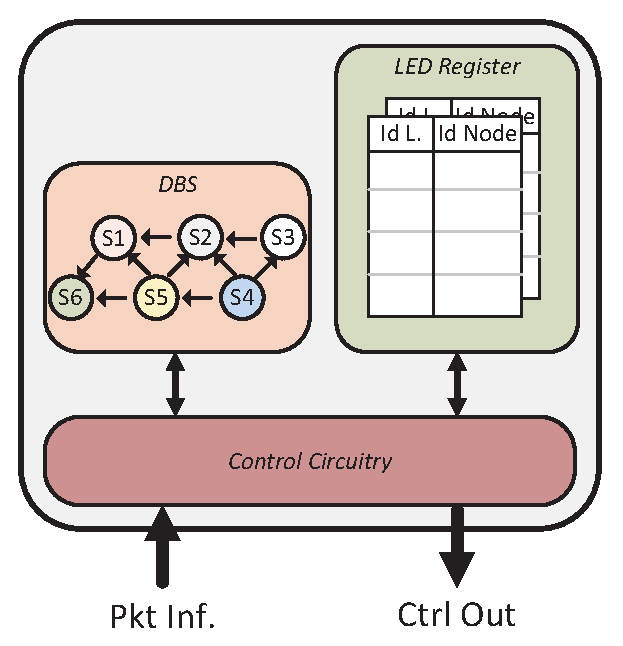
\includegraphics[width=0.35\textwidth]{pictures/disr_imp.eps}
  \caption{\emph{DiSR} block architecture.}
 \label{fig:implementation}
\end{figure}



Let us now look inside the \emph{DiSR} block which implements the DiSR-specific
operation. In Fig.~\ref{fig:implementation} is shown a possible sketch of this 
block, which mainly consist in the following building elements:

\begin{itemize}
\item \emph{DBS block}: It Takes trace of the dynamic behaviour status (DBS). 
      How discussed in the Sec.~\ref{ssec:disr_dstruct}, there are six possible status. 
      These status can be codified using only 3 bit implemented with a 3-bit register 
      and the required combinational logic. This block is essentially designed as a state machine.
\item \emph{LED register}: Is a set of register useful for storage the local environment data (LED)
      described in Sec.~\ref{ssec:disr_dstruct}. In Fig.~\ref{fig:implementation}, in their 
      respective block, are highlighted two table that represents the \emph{link\_visited[]} 
      and \emph{link\_tvisited[]}. The implementation of this block is an array of register 
      (one for each direction) that can be implemented with an SRAM, in which are presents two 
      specific fields  for representing the \emph{segID} (nodeID+linkID). 
\item \emph{Control circuitry}: This circuitry read the information from the incoming packet, 
      LED registers and the dynamic behaviour status (DBS block) and is able to write The LED
      informations and change the dynamic behaviour status. The output (Ctrl Out), drive 
      the others communications resources (such as node transceivers) for actuating the DiSR 
      routing operation.
\end{itemize}

One of the main design challenge typical of DNA Self-Assembled systems is due to the
reduced available resource  for implementing both computations and routing decisions for each node. 
The reason is the limited feasibility of DNA grids were can be placed the single unit cells such 
as CNFETs (carbon nanotube field-effect transistors) and nanowires.
For this reason, considering a budget of $10^4$ CNFETs for each network's node~\cite{liu_jetcs}
we should estimate the required resource for implementing the entire DiSR block 
(Fig.~\ref{fig:implementation}). For this purpose, after a description of the DiSR circuitry 
with an hardware description language (VHDL) we have synthesized at gate-level the required 
hardware. Furthermore, considering the specific layout of each single logic elements 
(such as NAND, full-adder, latch etc.), we are able to count the number of CNFETs 
necessary for implementing the DiSR logic. 
In particular, in Fig.\ref{fig:imp_trend} is shown the results of synthesis in therms 
of number of devices (CNFETs) versus the number of network nodes while the network scale 
up from $10\times10$ to $100\times100$ nodes. Can be observed that, while the node have
a squared increment, the circuitry complexity which implements the DiSR algorithm increase slowly. 
This means that the implemented system scale fine whit the number of network's node. 
For example, the increment of the number of register that implement the \emph{link\_visited[]} 
and \emph{link\_tvisited[]} table follow the function:

\begin{equation}
  \label{eq:imp_trend}
  N_{reg}=2\cdot N_{port} \cdot log_2(N)
\end{equation}
where $N_{port}$ is the number of the router's ports (4 in our cases), N is the number 
of network's node and the therms 2 take in account that \emph{link\_visited[]} and 
\emph{link\_tvisited[]} are two separate set o registers. While this number is fixed by 
the number of network's node, the control circuitry can be optimized applying more effort 
when designing this building block. However, observing the Fig.\ref{fig:imp_trend} can 
be pointed out that the proposed implementation occupy  about 20\% of the node budget. 

\begin{figure}
  \centering
  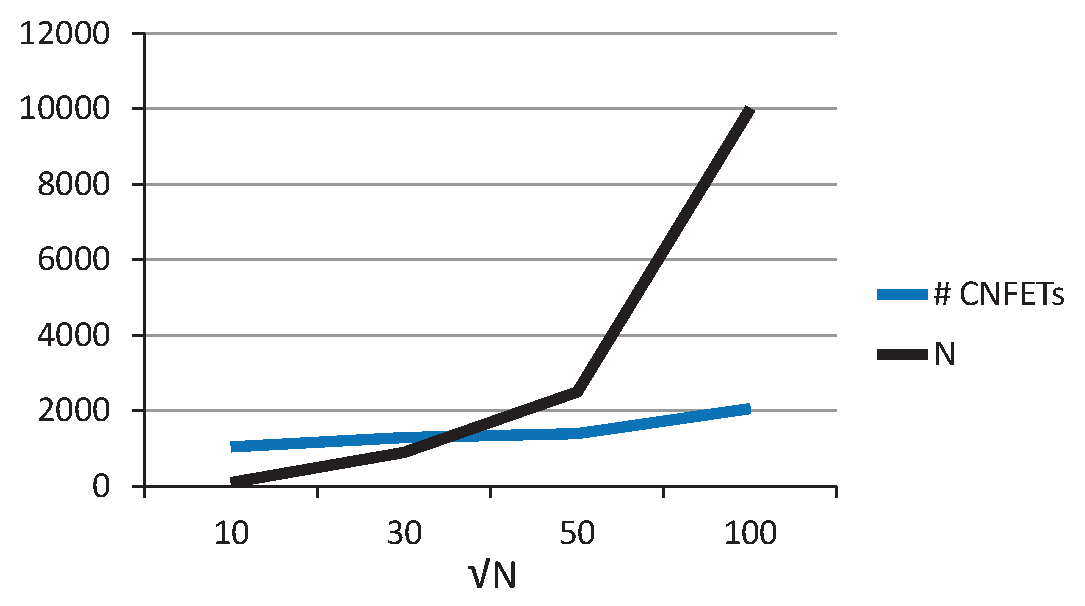
\includegraphics[width=0.48\textwidth]{pictures/imp_rslt.eps}
  \caption{DiSR synthesis results: N is the number of network's node.}
 \label{fig:imp_trend}
\end{figure}